\documentclass[reportComp]{thesis}
\usepackage[cpp,linenum,pseudo]{mypackage}

\title{并行分布式计算实验报告}
\subtitle{项目二:最短路径}
\school{数据科学与计算机学院}
\author{陈鸿峥}
\classname{17大数据与人工智能}
\stunum{17341015}
\headercontext{并行分布式计算实验报告}

\begin{document}

\maketitle

\section{题目描述}
现实世界的很多场景中,需要计算最短路径,如导航中的路径规划等,但是如何在大规模路径中快速找出最短路径,是一个具有挑战性的问题。
本项目要求利用MPI + OpenMP,从一个至少包含1万个节点,10万条边的图中,寻找最短路径,边上的权重可随机产生。
统一测试程序的执行时间,进行排名,根据排名计算成绩。

输入数据格式:
\begin{itemize}
	\item 20001个点,7000w+条边,求点0到点20000的最短路径(有解)
	\item 每行3个数,分别为源节点、汇节点、权重(非负)
\end{itemize}

输出:整个路径及路径长度

测试环境:3个节点(同主机的虚机),每个节点两个核心(双核四线程),4G内存,机械硬盘

参照:
\begin{itemize}
\item \url{https://github.com/Lehmannhen/MPI-Dijkstra}
\item \url{https://github.com/laplaceyc/Parallel-Programing}
\end{itemize}

\section{解决方案}
Dijkstra算法是串行求解单源最短路径的常见算法,伪代码如下
\begin{algorithm}[H]
\caption{Sequential Dijkstra SSSP}
\begin{algorithmic}[1]
\Procedure{Dijkstra}{Graph,Source}
\State Create vertex set $\sQ$\Comment{Initialization}
\For{\textbf{each} vertex in Graph}
\State dist[$v$] $\gets$ INFINITY
\State prev[$v$] $\gets$ UNDEFINED
\State add $v$ to $\sQ$
\EndFor
\State dist[$source$] $\gets$ $0$
\While{$\sQ$ is not empty}\Comment{Dijkstra}
\State $u$ $\gets$ vertex in $\sQ$ with min dist[$u$]
\State remove $u$ from $\sQ$
\For{\textbf{each} neighbor $v$ of $u$}
\State alt $\gets$ dist[$u$] + length($u$,$v$)
\If{alt $<$ dist[$v$]}\Comment{Relaxation}
\State dist[$v$] $\gets$ alt
\State prev[$v$] $\gets$ $u$
\EndIf
\EndFor
\EndWhile
\State\Return{dist[],prev[]}
\EndProcedure
\end{algorithmic}
\end{algorithm}

实际上,对于两个\verb'for each'部分,就可以使用并行方法进行加速,因为在循环间都没有依赖关系。
还有一个可并行的地方则是在求解距离最小值的部分(伪代码第9行)。

由于我现在的研究方向就是图计算,故本次作业直接复用了我今年以第一作者投稿于SC'19的部分代码,该代码是开源的\footnote{Krill: An Efficient Concurrent Graph Processing System, \url{https://github.com/chhzh123/Krill}}。

简单来说,优化技术有以下几点。
\begin{itemize}
	\item 将输入文件以字符串形式完全读入内存后,才并行进行处理,包括并行的初始化、并行的\textbf{基数排序}、并行的赋值等。
	\item 用\textbf{CSR(Compressed Sparse Row)格式}存储,见图\ref{fig:csr}
	\begin{figure}[H]
	\centering
	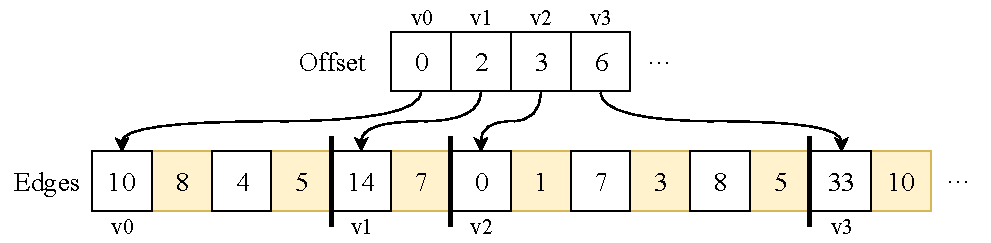
\includegraphics[width=0.8\linewidth]{fig/CSR.pdf}
	\caption{CSR格式}
	\label{fig:csr}
	\end{figure}
	其中,第一个数组存储的是边表的偏移量\verb'offset',第二个数组存储的是每个源结点的邻居(第一项)及边权(第二项)。
	以CSR格式存储,可以使程序具有良好的空间局部性。
	当确定了源结点(当前迭代最小距离点)后,内层循环都是遍历源结点的邻居。
	而在CSR格式中,邻居都是紧密存储的(包括边权),故这可以确保所需的数据都在Cache中,进而大大缩短访存时间。
\end{itemize}

头文件都在\verb'include'文件夹中,并行操作都已封装在\verb'parallel.h'头文件中(如OpenMP的\verb'parallel_for'等),主函数位于\verb'sssp.cpp'文件。

\section{实验结果}
运行可直接键入\verb'make run',结果如下(调用了Linux的\verb'time'函数进行计时)
\begin{lstlisting}[language=bash]
$time make run
./sssp 10001x10001GraphExamples.txt 20001
Dist: 2
20000<-826<-0

real    0m4.243s
user    1m26.519s
sys     0m19.259s
\end{lstlisting}

\end{document}